\documentclass[12pt]{article}
\usepackage{authblk}
\usepackage[english]{babel}
% or whatever
\usepackage[utf8]{inputenc}
\usepackage{times}
\usepackage{amssymb}
\usepackage{amsmath}
\usepackage{amsthm}
\usepackage{float}
\usepackage{graphicx}
\usepackage{subcaption}
\usepackage{floatflt}
%\usepackage{dsfont}	
%\usepackage{subscript}
\usepackage{enumitem}
\usepackage{amsbsy}
\usepackage{fixmath}
\usepackage{mathtools}
\usepackage{breqn}
\usepackage{booktabs}
\usepackage{hyperref}
\usepackage[english]{cleveref}
\usepackage{tabularx}
\usepackage{xcolor}
\usepackage{breqn}
\usepackage{fullpage}
\usepackage{tikz}

\usepackage{verbatim}

\usepackage{algorithm}
\usepackage[noend]{algpseudocode}

\parindent0pt

\hypersetup{
	colorlinks,
	citecolor=orange,
	filecolor=indigo,
	linkcolor=orange,
	urlcolor=blue
}


\DeclareMathOperator*{\argmin}{arg min}
\DeclareMathOperator*{\ds}{ds}

\begin{document}
	\author{Marcel A. Brusius,
			Leif Eric Goebel}
	\date{\today}
	\title{Results Exercise 2}
	\maketitle
	\begin{tikzpicture}[remember picture,overlay]
	\node [anchor=north west, inner xsep=0pt, inner ysep=0.455cm] at (current page.north west) {
\includegraphics[width=60mm]{Logo/tukl_logo_left.png}};
	\end{tikzpicture}	

	\begin{figure}
		\centering
		\begin{subfigure}{0.4\textwidth}
			\centering
			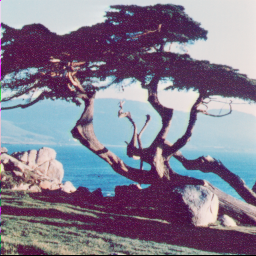
\includegraphics[width=0.8\textwidth]{tree/tree.png}
			\caption{Original}
		\end{subfigure}
		\begin{subfigure}{0.4\textwidth}
			\centering
			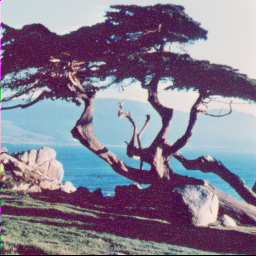
\includegraphics[width=0.8\textwidth]{tree/treetiffBilateralFilter.png}
			\caption{Bilateral}
		\end{subfigure}

		\begin{subfigure}{0.4\textwidth}
			\centering
			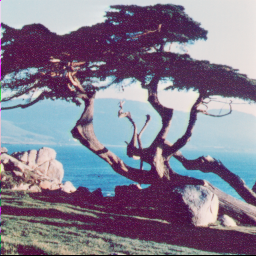
\includegraphics[width=0.8\textwidth]{tree/treetiffGuidedFilter.png}
			\caption{GuidedFilter}
		\end{subfigure}
		\begin{subfigure}{0.4\textwidth}
			\centering
			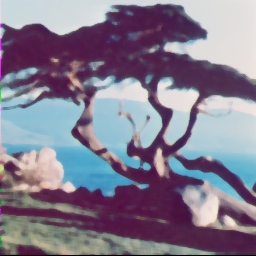
\includegraphics[width=0.8\textwidth]{tree/treetiffMedianFilter.png}
			\caption{Median}
		\end{subfigure}
	
		\begin{subfigure}{0.4\textwidth}
			\centering
			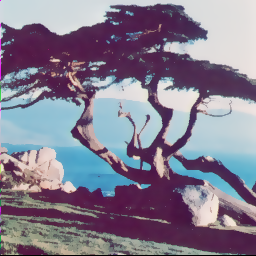
\includegraphics[width=0.8\textwidth]{tree/treetiffRollingGuidanceFilter.png}
			\caption{RollingGuidance}
		\end{subfigure}
		\caption{Landscape image}
	\end{figure}

	\begin{figure}
		\centering
		\begin{subfigure}{0.4\textwidth}
			\centering
			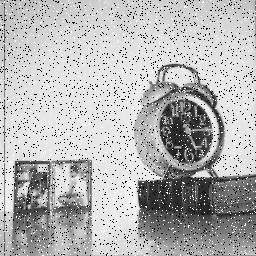
\includegraphics[width=0.8\textwidth]{saltandpepper/SaltAndPepper.png}
			\caption{Original}
		\end{subfigure}
		\begin{subfigure}{0.4\textwidth}
			\centering
			\includegraphics[width=0.8\textwidth]{saltandpepper/SaltAndPepperpngBilateralFilter.png}
			\caption{Bilateral}
		\end{subfigure}
		
		\begin{subfigure}{0.4\textwidth}
			\centering
			\includegraphics[width=0.8\textwidth]{saltandpepper/SaltAndPepperpngGuidedFilter.png}
			\caption{GuidedFilter}
		\end{subfigure}
		\begin{subfigure}{0.4\textwidth}
			\centering
			\includegraphics[width=0.8\textwidth]{saltandpepper/SaltAndPepperpngMedianFilter.png}
			\caption{Median}
		\end{subfigure}
		
		\begin{subfigure}{0.4\textwidth}
			\centering
			\includegraphics[width=0.8\textwidth]{saltandpepper/SaltAndPepperpngRollingGuidanceFilter.png}
			\caption{RollingGuidance}
		\end{subfigure}
		\caption{Salt and pepper noise image}
	\end{figure}

	\begin{figure}
		\centering
		\begin{subfigure}{0.4\textwidth}
			\centering
			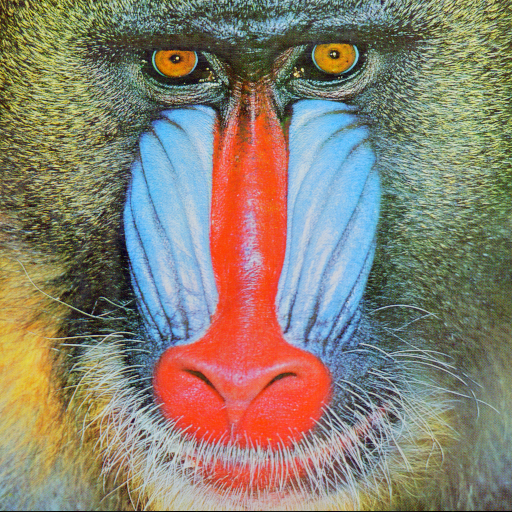
\includegraphics[width=0.8\textwidth]{mandrill/mandrill.png}
			\caption{Original}
		\end{subfigure}
		\begin{subfigure}{0.4\textwidth}
			\centering
			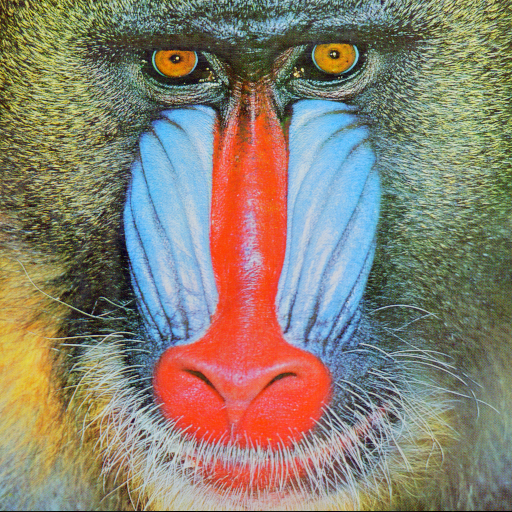
\includegraphics[width=0.8\textwidth]{mandrill/mandrilltiffBilateralFilter.png}
			\caption{Bilateral}
		\end{subfigure}
		
		\begin{subfigure}{0.4\textwidth}
			\centering
			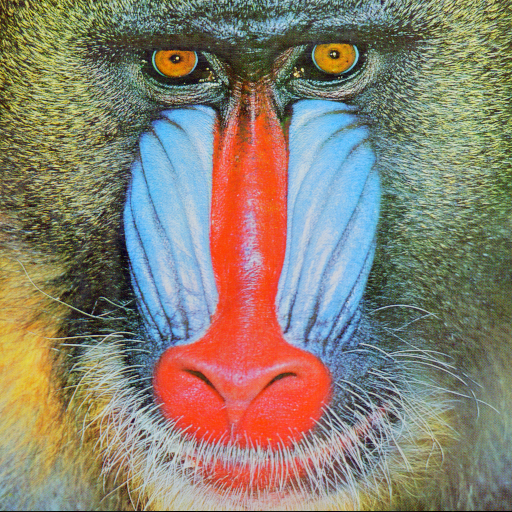
\includegraphics[width=0.8\textwidth]{mandrill/mandrilltiffGuidedFilter.png}
			\caption{GuidedFilter}
		\end{subfigure}
		\begin{subfigure}{0.4\textwidth}
			\centering
			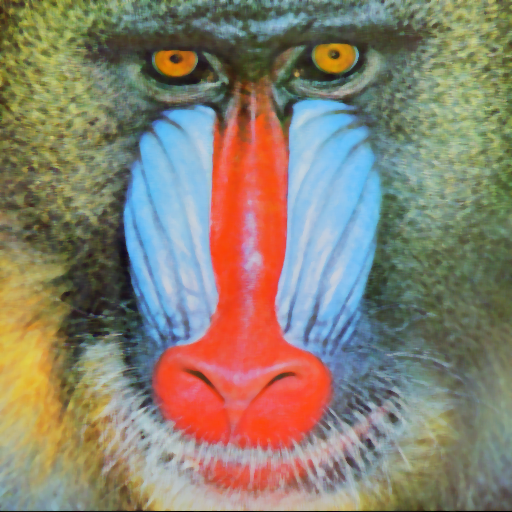
\includegraphics[width=0.8\textwidth]{mandrill/mandrilltiffMedianFilter.png}
			\caption{Median}
		\end{subfigure}
		
		\begin{subfigure}{0.4\textwidth}
			\centering
			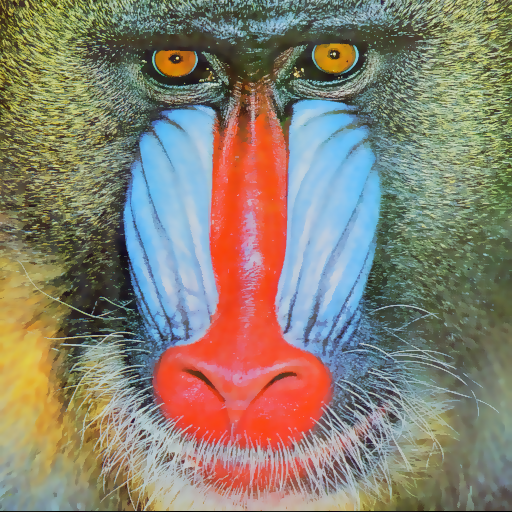
\includegraphics[width=0.8\textwidth]{mandrill/mandrilltiffRollingGuidanceFilter.png}
			\caption{RollingGuidance}
		\end{subfigure}
		\caption{Animal}
	\end{figure}
	
	\begin{figure}
		\centering
		\begin{subfigure}{0.4\textwidth}
			\centering
			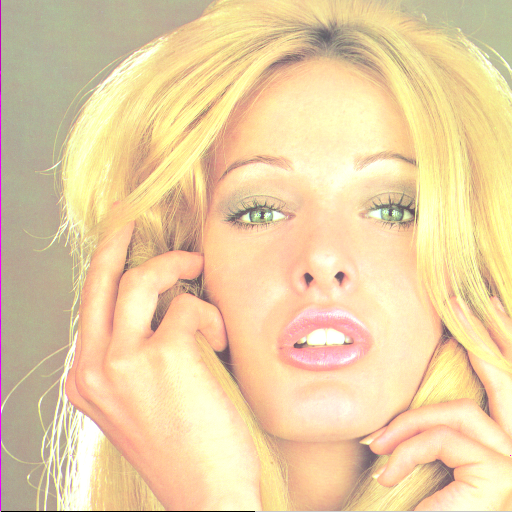
\includegraphics[width=0.8\textwidth]{tiffany/tiffany.png}
			\caption{Original}
		\end{subfigure}
		\begin{subfigure}{0.4\textwidth}
			\centering
			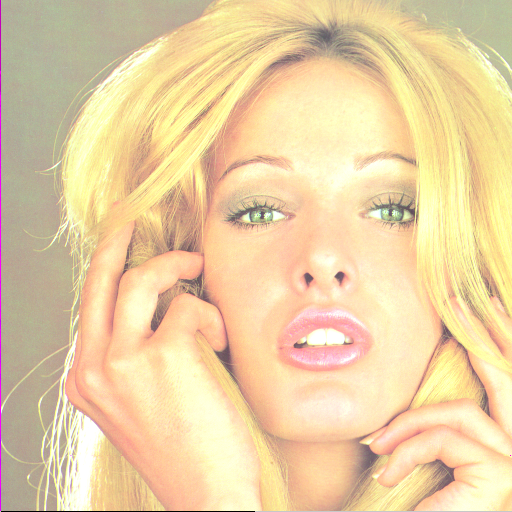
\includegraphics[width=0.8\textwidth]{tiffany/tiffanytiffBilateralFilter.png}
			\caption{Bilateral}
		\end{subfigure}
		
		\begin{subfigure}{0.4\textwidth}
			\centering
			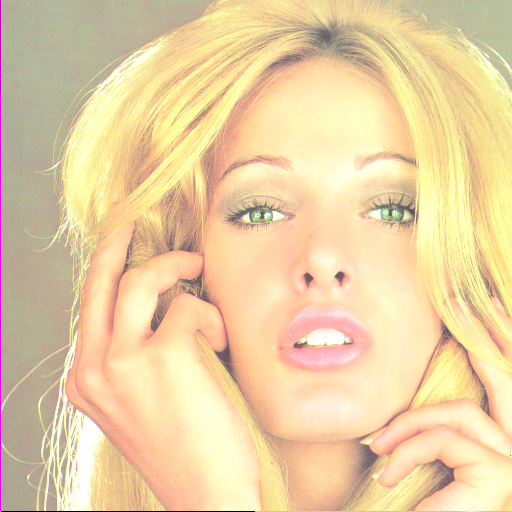
\includegraphics[width=0.8\textwidth]{tiffany/tiffanytiffGuidedFilter.png}
			\caption{GuidedFilter}
		\end{subfigure}
		\begin{subfigure}{0.4\textwidth}
			\centering
			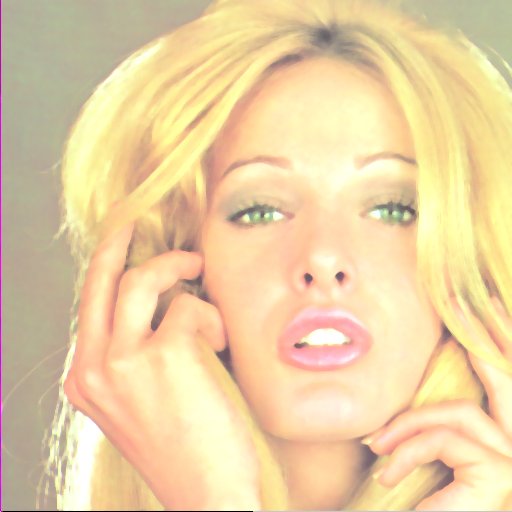
\includegraphics[width=0.8\textwidth]{tiffany/tiffanytiffMedianFilter.png}
			\caption{Median}
		\end{subfigure}
		
		\begin{subfigure}{0.4\textwidth}
			\centering
			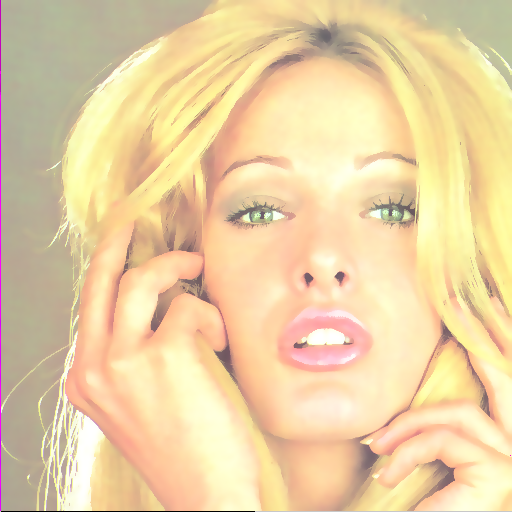
\includegraphics[width=0.8\textwidth]{tiffany/tiffanytiffRollingGuidanceFilter.png}
			\caption{RollingGuidance}
		\end{subfigure}
		\caption{Portrait}
	\end{figure}

	\begin{figure}
		\centering
		\begin{subfigure}{0.4\textwidth}
			\centering
			
\includegraphics[width=0.8\textwidth]{document/document.jpg}
			\caption{Original}
		\end{subfigure}
		\begin{subfigure}{0.4\textwidth}
			\centering
			
\includegraphics[width=0.8\textwidth]{document/documentjpgBilateralFilter.png}
			\caption{Bilateral}
		\end{subfigure}
		
		\begin{subfigure}{0.4\textwidth}
			\centering
			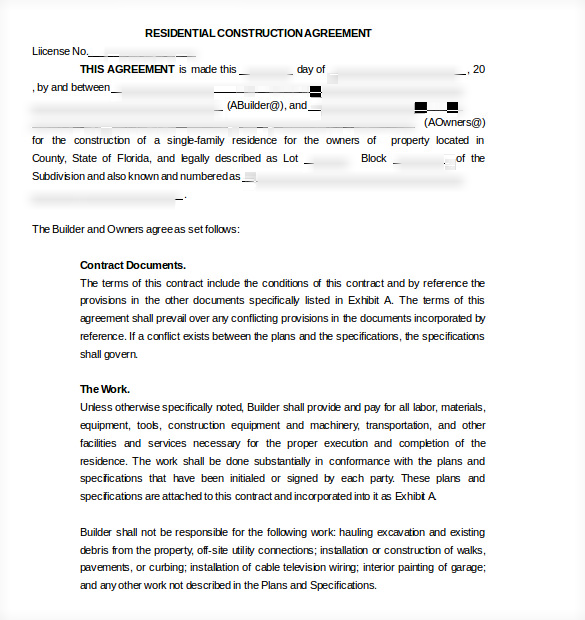
\includegraphics[width=0.8\textwidth]{document/documentjpgGuidedFilter.png}
			\caption{GuidedFilter}
		\end{subfigure}
		\begin{subfigure}{0.4\textwidth}
			\centering
			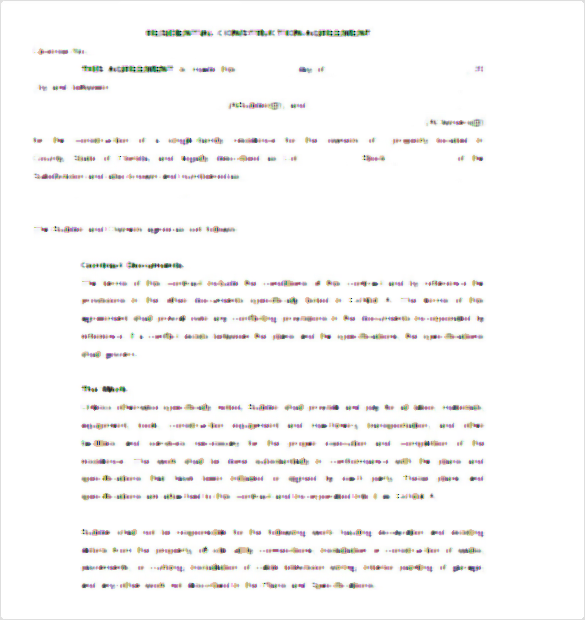
\includegraphics[width=0.8\textwidth]{document/documentjpgMedianFilter.png}
			\caption{Median}
		\end{subfigure}
		
		\begin{subfigure}{0.4\textwidth}
			\centering
			
\includegraphics[width=0.8\textwidth]{document/documentjpgRollingGuidanceFilter.png}
			\caption{RollingGuidance}
		\end{subfigure}
		\caption{Document}
	\end{figure}

	Bilateral filter was applied using $\sigma_C = 1.0, \sigma_S = 1.0$, Median filter used $k = 5.0$, guided filter was given $r = 5.0, \varepsilon = 0.001$ and rolling guidance filter used default values. Those choices were made in each set of sample images.
	
	\textbf{Exercise 1}\\
	\begin{itemize}
		\item[1)] The human eye automatically tries to amplify the contrast of colors. In this way the eye ``overcompensates'' the yellow veil of the image and the labels of the rubics cube appear blue. For the blue veil its the other way around. \\
		\item[2)] White balance is the effect of the surrounding light to the color values of an image. If most often changes the perception of white light and hence from all other colors in a similar way. The human brain adjusts this white balance automatically, whereas a camera can not do this. To adjust a camera one has to have an ``orientation'' area, which is supposed to be white. By applying a special filter, which uses the color value of the orientation area, one gets back a better result.\\
		\item[3)] We assume we have a mask or filter, which tells us, how exactly the heat diffuses from iteration $i$ to $i+1$. Then we can use the Fourier Transform of the image, apply the filter by multiplying the fourier coefficients and get a result for the next iteration by using the inverse fourier transformation. If the filter works in a way in which the normal heat equation works the image should get more equal after every iteration until it reaches a stationary point and does not change at all anymore.\\
		\item[4)] There are several filter, which we can apply. The easiest are e.g. mean and median filters. Others are bilateral and non-local filters. Both are a little bit more advanced, but also give better results. To maintain edges in an image (most often filter tend to blur the image a bit, but reduce noise) one has to take the edges itself into account and apply not only the filter but also edge detectors etc.\\
		\item[5)] The hysteresis threshold is a threshold for edge detectors, which ensures that and edge is only detected as edge, if the gradient is sufficiently large and which continues the edge beginning at the start. This way one gets only ``strong'' edges and keep them connected as long as it is possible.\\
		\item[6)] We think it should be possible to create an algorithm, which nearly draws lines as humans does, but not exactly like humans would do. The problem is to quantify and qualify the edges. Each human would draw lines in a different way. In the paper they averaged over all drawings they had to somewhat quantify the lines. This is a nice approach, but still just ``approximate'' the lines drawn.
	\end{itemize}
\end{document}
